%%%%%%%%%%%%%%%%%%%%%%%%%%%%%%%%%%%%%%%%%%%%%%%%%%%%%%%%%%%%%%%%%%%%%%%%%%%%%%%%
% Template for USENIX papers.
%
% History:
%
% - TEMPLATE for Usenix papers, specifically to meet requirements of
%   USENIX '05. originally a template for producing IEEE-format
%   articles using LaTeX. written by Matthew Ward, CS Department,
%   Worcester Polytechnic Institute. adapted by David Beazley for his
%   excellent SWIG paper in Proceedings, Tcl 96. turned into a
%   smartass generic template by De Clarke, with thanks to both the
%   above pioneers. Use at your own risk. Complaints to /dev/null.
%   Make it two column with no page numbering, default is 10 point.
%
% - Munged by Fred Douglis <douglis@research.att.com> 10/97 to
%   separate the .sty file from the LaTeX source template, so that
%   people can more easily include the .sty file into an existing
%   document. Also changed to more closely follow the style guidelines
%   as represented by the Word sample file.
%
% - Note that since 2010, USENIX does not require endnotes. If you
%   want foot of page notes, don't include the endnotes package in the
%   usepackage command, below.
% - This version uses the latex2e styles, not the very ancient 2.09
%   stuff.
%
% - Updated July 2018: Text block size changed from 6.5" to 7"
%
% - Updated Dec 2018 for ATC'19:
%
%   * Revised text to pass HotCRP's auto-formatting check, with
%     hotcrp.settings.submission_form.body_font_size=10pt, and
%     hotcrp.settings.submission_form.line_height=12pt
%
%   * Switched from \endnote-s to \footnote-s to match Usenix's policy.
%
%   * \section* => \begin{abstract} ... \end{abstract}
%
%   * Make template self-contained in terms of bibtex entires, to allow
%     this file to be compiled. (And changing refs style to 'plain'.)
%
%   * Make template self-contained in terms of figures, to
%     allow this file to be compiled. 
%
%   * Added packages for hyperref, embedding fonts, and improving
%     appearance.
%   
%   * Removed outdated text.
%
%%%%%%%%%%%%%%%%%%%%%%%%%%%%%%%%%%%%%%%%%%%%%%%%%%%%%%%%%%%%%%%%%%%%%%%%%%%%%%%%

% \documentclass[letterpaper,twocolumn,10pt]{article}
\documentclass[sigplan, 10pt]{acmart}
%\documentclass[letterpaper,twocolumn,10pt]{acmart}

\AtBeginDocument{%
  \providecommand\BibTeX{{%
    \normalfont B\kern-0.5em{\scshape i\kern-0.25em b}\kern-0.8em\TeX}}}
    

% to be able to draw some self-contained figs
\usepackage{tikz}
\usepackage{amsmath}

% inlined bib file
\usepackage{filecontents}

\usepackage{times}
\usepackage{datetime}
\usepackage{url}
\usepackage{hyperref}

\usepackage[normalem]{ulem}
\usepackage{multirow}
\usepackage{comment}
\usepackage{listings}
\usepackage{tikz}
\usepackage{verbatimbox}
\usepackage{amssymb}
\usepackage{pifont}
\usepackage{booktabs}
\usepackage[keeplastbox]{flushend}
\usepackage{enumitem}
\usepackage{caption}

\newcommand*\circled[1]{\tikz[baseline=(char.base)]{
            \node[shape=circle,draw,inner sep=1pt] (char) {\small #1};}}

\newcommand{\todo}[1]{{\color{red}\bfseries [[#1]]}}
\newcommand{\XZ}[1]{{\color{blue}\bfseries [[#1]]}}
\newcommand{\TP}[1]{{\color{red}\bfseries [[#1]]}}
\newcommand{\HG}[1]{{\color{magenta}\bfseries [[#1]]}}
\newcommand{\NP}{\texttt{NumaPerf}}
\newcommand{\specialcell}[2][c]{%
  \begin{tabular}[#1]{@{}c@{}}#2\end{tabular}}
  \newcommand{\TM}{\text{thread migration}}
  \newcommand{\PS}{\text{remote access}}
  \newcommand{\TS}{\text{true sharing}}
  \newcommand{\FS}{\text{false sharing}}
  \newcommand{\TI}{\text{thread imbalance}}   \newcommand{\TB}{\text{thread binding}}
  \newcommand{\BI}{\text{block interleave}}
  \newcommand{\PI}{\text{page interleave}}
  \newcommand{\PAD}{\text{padding}}
  \newcommand{\DUP}{\text{duplicate}}




\begin{document}
%-------------------------------------------------------------------------------

%don't want date printed
\date{}

% make title bold and 14 pt font (Latex default is non-bold, 16 pt)
%\title{\Large \bf Formatting Submissions for a USENIX Conference:\\
%  An (Incomplete) Example}
%\title{NUMAPerf: Predictive and Comprehensive NUMA Profiling}
\title{NumaPerf: Predictive and Comprehensive NUMA Profiling}

%for single author (just remove % characters)
%\author{
%{\rm Your N.\ Here}\\
%Your Institution
%\and
%{\rm Second Name}\\
%Second Institution
% copy the following lines to add more authors
% \and
% {\rm Name}\\
%Name Institution
%} % end author

% Authors: Xin Zhao, Jin Zhou, Hui Guan, Xu Liu, Wei Wang, Tongping Liu


%-------------------------------------------------------------------------------
\begin{abstract}
We are planning to work on a NUMA performance detector--\NP{}. Different from existing allocators, \NP{} focuses on memory sharing pattern, and identify objects that have a large number of accesses from different threads. The difference is that the detection results are not relied on the current hardware topology, which can find potential performance issues for any topology. This will avoid the endless detection on different hardware.

We will compute the potential performance issue during the offline diagnosis, while only those shared ones will be identified.    

\end{abstract} 

\maketitle

\section{Introduction}
\label{sec:intro}

The Non-Uniform Memory Access (NUMA) is the de facto  design to address the scalable issue of an increased number of hardware cores. Compared to the Uniform Memory Access (UMA) architecture, the NUMA architecture avoids the bottleneck of one memory controller by allowing each node/processor to concurrently access its own memory controller. However, the NUMA architecture imposes multiple system challenges for writing efficient parallel applications, such as remote accesses, interconnect congestion, and node imbalance~\cite{Blagodurov:2011:CNC:2002181.2002182}. User programs could easily suffer from significant performance degradation, necessitating the development of profiling tools to identify NUMA-related performance issues. 

General-purpose profilers, such as \texttt{gprof}~\cite{DBLP:conf/sigplan/GrahamKM82}, \texttt{perf}~\cite{perf}, or \texttt{Coz}~\cite{Coz}, are not suitable for identifying NUMA-related performance issues~\cite{XuNuma,valat:2018:numaprof} because they are agnostic to the architecture difference. 
%Existing NUMA-related profiling tools can be largely classified into three types. One 
To detect NUMA-related issues, one type of tools
simulates cache activities and page affinity based on collected memory traces~\cite{NUMAGrind, MACPO}. However, they may introduce hundreds or even thousands of performance slowdown, preventing their uses even in development phases. In addition to this, one type employs coarse-grained sampling to identify performance issues in the deployment environment~\cite{Intel:VTune, Memphis, Lachaize:2012:MMP:2342821.2342826, XuNuma, NumaMMA, 7847070}, while the other type builds on fine-grained instrumentation that could detect more performance issues but with a higher overhead. Among them, profiling-based tools may miss some performance opportunities, and provide misleading information for fixes.  
%Due to this fact, fine-grained tools are more suitable for the development phase, which aims to detect as many performance issues as possible before the release of software. 

%\todo{Do existing work differentiate false sharing and true sharing? This is important since false sharing and true sharing will require different fixes, and most true-sharing can be very difficult to fix} 

However, the later two types of existing tools share the following \textbf{common issues}. \textit{First, they have the portability issue. They can only identify performance issues on the current NUMA hardware}. Typically, they rely on the actual node information to detect a remote access: a remote access happens when the physical memory a thread accesses is located in a remote node that is different from the one that the thread is running on. However, they cannot uncover remote accesses with a different hardware topology. Further, some  tools explicitly bind threads to cores~\cite{XuNuma}, which may miss some remote accesses caused by the binding. \textit{Second, they suffer from the effectiveness issue, leading to the miss of many optimization opportunities}. They only focus on one type of remote accesses, while omitting other reasons (e.g., thread migration) that could also incur remote accesses. Further, they omit load imbalance, another source of performance degradation. As a result, they could only detect a small portion of performance issues, as shown in our evaluation. \textit{Third, existing tools could not provide sufficient guidelines for bug fixes}. This will leave significant burden for users in order to figure out a suitable fix strategy. For instance, they cannot report whether remote accesses are caused by true or false sharing that clearly requires different fix strategy.   


This paper proposes a novel tool---\NP{}---that overcomes all of these existing issues. \NP{} is designed as an automatic tool that does not require human annotation or the change of the code. It also does not require new hardware, or the change of the underlying operating system. \NP{} aims to detect  NUMA-related issues in the development phase, when applications are exercised with representative inputs. In this way, there is no need for paying additional runtime overhead in deployment phase. We further describe \NP{}'s distinctive features in the following. 

First, \NP{} proposes a predictive mechanism that could detect performance issues for any NUMA architecture, even without running on a NUMA architecture. It is based on a \textbf{key observation} that \textit{a thread may run on any physical node due to the scheduling}. Based on this observation, \NP{} tracks the relationship between memory accesses and threads, instead of physical nodes. It greatly simplifies the detection problem: there is no need to know the node on which a thread is running; there is also no need to track the physical node information for each page. Instead, \NP{} only tracks sharing pattern of memory accesses. The observation also makes it possible to detect all potential issues within development phases, instead of paying unnecessary runtime overhead in a deployment environment, assuming applications are fed with representative inputs. 


Second, \NP{} will significantly increase the detection effectiveness by identifying more types of NUMA performance issues. \NP{} detects remote accesses caused by cross-node thread migrations, one issue omitted by all existing tools. Based on our evaluation, cross-node migration may lead to $4\times$ performance degradation for \texttt{fluidanimate}, since it basically turns all previous local accesses into remote accesses. 
%A migrated thread is forced to reload its data that already exists in its previous cache, and access its stack and pages remotely. Further, it will also disrupt memory allocations to create non-local allocations, since most existing allocators will not return freed objects to its original node. 
\NP{} also detects load imbalances among threads, which may lead to memory controller congestion and interconnect congestion. 
%It instruments all memory accesses in order to predict the load imbalance correctly. 
%As mentioned above, applications may suffer significant performance issues due to remote accesses, memory controller congestion, and interconnect congestion, but existing tools detect only partial issues related to remote accesses. Based on our understanding, memory controller congestion and interconnection congestion are also related with load imbalance. Therefore, 
%\NP{} extends its detection scope to identify both remote accesses and load imbalance. For remote accesses, 

Last but not least, \NP{} aims to provide sufficient information that helps bug fixes. For remote accesses caused by sharing, \NP{} will differentiate  cache-level sharing from page-level sharing, and false sharing from true sharing, since different sharing patterns will have different fix strategies. For instance, padding can easily fix cache-level false sharing but is impractical for page-level false sharing or true sharing. If remote accesses are caused by thread migration, \NP{} will suggest thread binding. For load imbalance, \NP{} will suggest the number of threads in order to balance workloads. 
%thread clustering for particular threads and the adjusting number for each type of threads in order to balance workloads.   

%We discovered that applications with a high number of system calls or synchronizations will have a high potential to have thread migration. That is due to the reason that a thread will be placed into a waiting queue, upon synchronizations or system calls, then it could be migrated to a different node by the OS scheduler.


We have performed extensive evaluations to verify the effectiveness of \NP{} with widely-used parallel applications (i.e., PARSEC~\cite{parsec}) and HPC applications (e.g., Lulesh, AMG2006, and UMT2003).  \NP{} detects many more performance issues than the combination of all existing NUMA profilers, including both fine-grained and coarse-grained tools. After fixing these issues, these applications could achieve up to $5.94\times$ performance improvement. Further, \NP{} also provides sufficient information for bug fixes, which is exemplified by few case studies. 
%We further evaluates \NP{}'s performance and memory overhead. \NP{} introduces around $X\times$ performance overhead and 

Overall, \NP{} makes the following contributions. 

\begin{itemize}
    \item \NP{} is the first tool that could predictively detect NUMA-related performance issues without relying on a specific NUMA architecture. 
    \item \NP{} proposes multiple mechanisms to detect a comprehensive set of NUMA-related performance issues, including those caused by thread migration and load imbalance but omitted by existing tools. 
    \item \NP{} provides helpful information to assist bug fixes, which is lacked in existing tools. 
    \item We have performed extensive evaluations to confirm \NP{}'s effectiveness and overhead.  
\end{itemize}


\subsection*{Outline}

The remainder of this paper is organized as follows. Section~\ref{sec:overview} introduces the background of NUMA architecture and the basic idea of \NP{}. Then Section~\ref{sec:implementation} presents the detailed implementation and Section~\ref{sec:evaluation} shows experimental results. In the end, Section~\ref{sec:related} discusses related work in this field, and Section~\ref{sec:conclusion} concludes this paper.

\begin{comment}
 Existing work is typically bound to a specific architecture. 
 
 In addition, they could only identify one type of issue that a NUMA issue inside the application. However, they cannot explain whether a NUMA issue is caused by the allocator. 
 
 We observe that NUMA performance issue is similar to cache contention, but can occur in both cache and page granularity. Therefore, we could utilize the same framework to identify both cache contention (false/true sharing) and page-level false sharing issue, instead of only on the page granularity. 
 
 We also observe that existing profilers only work on a particular architecture. 
 
 Third, existing profilers could not identify the issues caused by the allocator, which makes them cannot explain performance issue of an allocator. 
 
 
 \NP{} will have the following differences. 
 \begin{itemize}
 \item \NP{} does not rely on a specific hardware, which could identify issues in any potential hardware. 
 \item \NP{} could identify the issue caused by the memory allocator, such as passive and active false sharing of objects. 
 \item \NP{} could even identify the metadata issues of a memory allocator. 
 \item \NP{} could identify both cache and page sharing, where both of them have a significant performance impact on the application. 
 \end{itemize}

 


Our work is to derive some potential problems of existing applications on the given NUMA hardware, then provides an insight to users how to solve the problem by fixing existing applications. And our work will utilize the on-line analysis. 

% see the paper: Toward the efficient use of multiple explicitly managed memory subsystems.
In this paper, we use emulator-based profiling to analyze actual program executions when programs are executed, this setup allows us to associates the cache misses with the different memory objects of the executed application. 
This paper shares the similar target as our paper. 

~\cite{Bolosky:1989:SBE:74850.74854} is their original work that talks about the page management. 


We observe that the number of cache loading is the most important metrics.
In order to evaluate the performance impact, we propose to utilize the number of cache invalidations to evaluate the seriousness of NUMA issues. A more intuitive metrics is the cache line loading operations. However, it is impossible to do this very easily. Thus, we proposes to utilize the number of cache invalidation as the metrics. 


However, cache invalidations can be affected by two factors: cache-line based sharing, and size-related invalidations. 
Size-related invalidations indicate that one core's cache is not sufficient to cover the memory footprint of the thread. Therefore, some cache lines will be evicted, which will cause cause invalidation. However, it is not easy to do this, which will be omitted by the \NP{}. 

Instead, \NP{} focuses cache invalidations caused by sharing, either true or false sharing. Similarly, page-level sharing will end up with the same issue, due to the existence of cache. If the data is held in the cache line and the data is valid, then there will be no remote accesses even if the actual physical page is located remotely. 

Therefore, we propose \NP{} to be a profiling tool that could identify both page and cache-level sharing. Also, \NP{} is based on the observation that applications may have performance issue even if it does not in the current architecture. 

However, the challenge is to evaluate the number of cache invalidations correctly and efficiently. Predator also utilizes the similar mechanism, but cannot compute the number correctly. Then we will give an example about this. 

\NP{} instead will compute the number differently. It will has the number of copies for all threads for each thread, and then the detailed information for each word (which helps to solve the issue). For each write operation, we will increment the number of copies correspondingly, instead of just one.

However, there will be some efficiency issue on the performance and the memory. We can't have the information for each cache line, which will at least impose around $2\times$ memory overhead. Also, we could easily cause significant performance issue if we have to traverse the cache line for all memory writes. 
 
\todo{Should we traverse the whole cache line? Or we will use the word-based structure? Then when there is invalidation, then we will clean the per-line flag. } Then we will guarantee that every access will only invoke $O(1)$ operations. 


To reduce the memory overhead, we will utilize the number of cache misses and the number of threads as a metrics. If a cache line is only accessed by one thread, then it is possibly only accessed by a thread, then it should not cause the performance issue. 
Also, if the number of writes on a cache line is small, it will never be the performance issue for most cases. 

However, we may need to save the number of cache misses for each callsite together. Otherwise, some objects will be skipped. 


\NP{} is different from existing work that it also profiles the performance issue caused by allocators.  

Major difference:

1. MACPO focus on the code with identified bottleneck, not the whole program.
2. MACPO only works on arrays, unions, structures, not all variables. 
3. They care about reuse-distance, and XXX. We may only care about the number of remote accesses
4. They use offline analysis, not sure whether that is one of reason that cause substantial overhead sinceit will have tons of IO operations. We don't know whether the analysis online will have a better performance
5. MACPO only output the reuse distance, remote access number, cycles per access (because they utilize the cycle-based cache simulation), access strides (for prefetching). They have output like Figure2. 

\end{comment}
 






\section{Overview}

\subsection{NUMA Architecture}
\label{sec:numa}

Traditional computers use the Uniform Memory Access (UMA) model. In this model,  all CPU cores share a single memory controller such that any core can access the memory with the same latency (uniformly). However, the UMA architecture cannot accommodate the increasing number of cores in recent years because these cores may compete for the same memory controller. The memory controller becomes the performance bottleneck in many-core machines since a task cannot proceed without getting its necessary data from the memory. 

The Non-Uniform Memory Access (NUMA) architecture is proposed to solve the scalability issue. It has a decentralized nature. Instead of making all cores waiting for the same memory controller, the NUMA architecture  is typically equipped with multiple memory controllers, where each controller serves a group of CPU cores (called as a node). Incorporating multiple memory controllers largely reduce the contention for memory controllers and therefore improve the scalability correspondingly. However, the NUMA architecture also introduce multiple sources of performance degradations~\cite{Blagodurov:2011:CNC:2002181.2002182}, including \textit{Cache Contention}, \textit{Node Imbalance}, \textit{Interconnect Congestion}, and \textit{Remote Accesses}. 

\textbf{Cache Contention:} the NUMA architecture is prone to cache contention: multiple tasks may compete for the shared cache. Cache contention will cause more serious performance degradation if data has to be loaded from a remote node. 
 
\textbf{Node Imbalance:} When some memory controllers have much more memory accesses than others, it may cause the node imbalance issue. Therefore, some tasks may wait more time for memory accesses, thwarting the whole progress of a multithreaded application.  

\textbf{Interconnect Congestion:} Interconnect congestion occurs if some tasks are placed in remote nodes that may use the inter-node interconnection to access their memory. 

\textbf{Remote Accesses:} In NUMA architecture, local nodes can be accessed with less latency than remote accesses. Therefore, it is important to reduce remote accesses to improve the performance.\\


 Based on the study~\cite{Blagodurov:2011:CNC:2002181.2002182}, node imbalance and interconnect congestion may have a larger performance impact than cache contention and remote accesses. These performance issues cannot be solved solely by hardware design. Software support is required to control the placement of tasks, physical pages, and objects to achieve the optimal performance for multithreaded applications.  
 
\subsection{Basic Idea}

Fine-grained profiling (compiler-based instrumentation) 

Detection: 
Remote accesses [thread-based design, potential node migration ]

If there are too many migrations, then we will use the binding. 

The binding will be related with node imbalance. 

Load imbalance: 
Identify number of memory accesses from each thread. 
(1) Find applications that should use binding. 
(2) Find how to bind threads together. 
(3) Find how to change the number of threads to achieve better balance. 


\section{Design and Implementation}
\label{sec:implementation}

This section elaborates \NP{}-Static and \NP{}-Dynamic. \NP{} leverages compiler-based instrumentation (\NP{}-Static) to insert a function call before memory access, which allows \NP{}-Dynamic to collect memory accesses. \NP{} utilizes a pre-load mechanism to intercept synchronizations and memory allocations, without the need of changing programs explicitly. Detailed design and implementation are discussed as follows. 

\begin{comment}
\NP{} leverages compiler-based instrumentation to insert a handle function for each memory access. This allows \NP{} to collect memory accesses.
how the memory is accessed in both page and cache level, and collect the sharing pattern when the memory object is freed by users.If they are never freed explicitly, \NP{} can do the collection in the end of the whole application. If too many remote memory access happened in a memory object, it needs an attention. Besides, \NP{} also collected thread based information like how many thread migration happened, how many different thread groups, and how many local and remote memory access incurred in each thread.Based on these thread based information, \NP{} could tell users what kinds of NUMA imbalance issues the application contained and how to fix it.

\end{comment}

\subsection{\NP{}-Static} 
\NP{}'s static component (\NP{}-Static) performs the instrumentation on memory accesses. In particular, it utilizes static analysis to identify memory accesses on heap and global variables, while omitting memory accesses on static variables. Based on our understanding, static variables will never cause performance issues, if a thread is not migrated. \NP{}-Static inserts a function call 
upon these memory accesses, where this function is implemented in \NP{}-Dynamic library. In particular, this function provides detailed information on the access, including the address, the type  (i.e., read or write), and the number of bytes.  

\NP{} employs the LLVM compiler to perform the instrumentation~\cite{llvm}. It chooses the intermediate  representation (IR) level for the instrumentation due to the flexibility, since LLVM provides lots of APIs and tools to manipulate the IR. The instrumentation pass is placed at the end of the LLVM optimization passes, where only memory accesses surviving all previous optimization passes will be instrumented.  \NP{}-Static traverses functions one by one, and instruments memory accesses on global and heap variables. The instrumentation is adapted from AddressSanitizer~\cite{AddressSanitizer}.
%, which drastically reduce the number of function calls due to its static analysis and the placement of the instrumentation inside optimization passes. 

\begin{comment}

To intercept memory access instructions, The function call is implemented by \NP{}, through which \NP{} could intercept each memory access operation from target applications with its address and access type(read or write).

It is worth to note that \NP{} only focused on memory access to heap objects and global objects, since they have much higher chance to be shared for multiple threads, which leads potential NUMA issues. If an object is only accessed by one single thread, it will never cause performance issues, unless threads migrated to another nodes and \NP{} could also detect this problem that is detailed described in the following parts.Besides, the pass function should be placed at the very end of compiling optimization phase of LLVM, since most memory access instructions will be optimized out after huge amounts of compiling optimization strategies applied by LLVM. Based on our experiments, the number of memory access instructions could be reduce by half or more.So if the order of the pass function is not set properly, huge amounts of duplicated instrumentation calls will be made which not only brings more overheads but also makes the profiling results not accurate.

\end{comment}

% What are the challenges of that? 
% What type of issues that we usually have. I remembered that we used to have high overhead with compiler-based instrumentation.

% What particular issue for the version of instrumentation. 

\subsection{\NP{}-Dynamic}

This subsection starts with tracking application information, such as memory accesses, synchronizations, and memory allocations. Then it discusses the detection of each particular performance issue.  In the following, \NP{} is used to represent \NP{}-Dynamic unless noted otherwise. 

\subsubsection{Tracking Accesses, Synchronizations, and Memory Allocations}

\NP{}-Dynamic implements the inserted functions before memory accesses, allowing it to track memory accesses. Once a memory access is intercepted, \NP{} performs the detection as discussed below. 

\NP{} utilizes a preloading mechanism to intercept synchronizations and memory allocations before invoking correspond functions.
%It implements all synchronization functions related to mutexes, condition variables, and thread creations, as well as memory allocations and deallocations. 
%By forcing the pre-loading the \NP{}-Dynamic, we are able to intercept these functions before their actual invocations. 
\NP{} intercepts synchronizations in order to detect possible thread migrations, which will be explained later. \NP{} also intercepts memory allocations, so that we could attribute performance issues to different callsites, assisting data-centric analysis~\cite{XuNuma}. For each memory allocation, \NP{} records the allocation callsite and its address range. 
%Currently, \NP{} obtains the callsite of the allocation from the stack directly.  
\NP{} also intercepts thread creations in order to set up per-thread data structure. 
In particular, it assigns each thread a thread index.

%each thread will be assigned a thread index that starts with 0, which will be incremented upon each new thread creation. The thread index of each thread will be stored in thread-local storage in order to obtain it quickly. 

\subsubsection{Detecting Normal Remote Accesses}
\label{sec: remote_access}

%As discussed in Section~\ref{sec:numa},  a large number of remote accesses is the most common reason for the performance issue on the NUMA architecture, which is the focus of existing NUMA profilers~\cite{XuNuma, valat:2018:numaprof}. Existing work detects a remote access if the current thread is running on a physical node that is different from the physical node of the corresponding page. However, they impose additional overhead of determining the physical node of each page and each thread. Also, they could only detect remote accesses occurring in the evaluated machine, which is architecture-dependent. 

%As discussed in Section~\ref{sec:numa}, 
%Instead of basing on the physical node relationship, \NP{} proposes an architecture-independent mechanism that does not require the actual node relationship.
\textit{\NP{} detects a remote access when an access's thread is different from the corresponding page's initial accessor}, as discussed in Section~\ref{sec:overview}. This is based on the assumption that the OS typically allocates a physical page from the node of the first accessor due to the default first-touch policy~\cite{firsttouch}.  Similar to existing work, \NP{} may over-estimate the number of remote accesses, since an access is not a remote one if the corresponding cache is not evicted. 
%The over-estimation may generate false alarms that may report non-serious NUMA issues.  
However, this shortcoming can be overcome easily by only reporting issues larger than a specified threshold, as exemplified in our evaluation (Section~\ref{sec:evaluation}).  

\NP{} is carefully designed to reduce its performance and memory overhead.  \NP{} tracks a page's initial accessor to determine a remote access. A naive design is to employ hash table for tracking such information.%, which will  be checked upon each memory access. 
Due to a large number of memory accesses, a naive design (e.g. hash table) could easily introduce significant performance overhead. 
Instead, \NP{} maps a continuous range of memory with the shadow memory technique~\cite{qinzhao}, which only requires a simple computation to locate the data. 
%Specifically, \NP{} predicts the maximum range for heaps (e.g. 4TB) and globals, and then maps a continuous range of memory to store the owner of each page. 
%For each access, \NP{} requires only a simple computation to locate the corresponding data. 
%As described above, since \NP{} aims to provide data-centric information that helps users pinpoint susceptible objects with extensive remote accesses, it should determine the corresponding pages and objects. To assist this, 
\NP{} also maintains the number of accesses for each page in the same map. 
%Upon each memory access, \NP{} simply increments the number of access for the corresponding page. \NP{} further utilizes the sampling mechanism to reduce the overhead, which only updates remote accesses for \todo{one out of 100 accesses}. 
We observed that a page without a large number of memory accesses will not cause significant performance issues. Based on this, \NP{} only tracks the detailed accesses for a page, when its number of accesses is larger than a pre-defined (configurable) threshold. 
%That is, \NP{} does not track the detailed information for most pages. In order to differentiate these pages, \NP{} stores a pointer in the same map that points to the detailed information for some pages. 
Since the recording uses the same data structures, \NP{} uses an internal pool to maintain such data structures with the exact size, without resorting to the default allocator.  
%\todo{Maybe too much on this?? Due to the performance concern, \NP{} avoids the use of the default allocator for these data structures.  Instead, \NP{} designs a slab-like allocator that keeps a pool of objects. }  

For pages with excessive accesses, \NP{} tracks the following information. \textit{First}, it tracks the threads accessing these pages, which helps to determine whether to use block-wise allocations for fixes. 
%\todo{For instance, if only two threads access the same page continuously, then we could utilize a block-wise allocation and bind these two threads to the same physical node in order to achieve the better performance}. The detailed fixing strategy is out of the scope, but Section~\ref{sec:casestudies} provides multiple examples. 
\textit{Second}, \NP{} further 
divides each page into multiple blocks (e.g., 64 blocks), and tracks the number of accesses on each block.  
%records the corresponding access number. Such information will be helpful for data-centric attribution, since an object may only cover part of some pages. 
This enables us to compute the number of remote accesses of each object more accurately. \textit{Third}, \NP{} further checks whether an object is exclusively read after the first write or not, which could be determined whether duplication is possible or not. 
%is good to duplicate the data to multiple nodes. Read-exclusively objects can be duplicated to different nodes, in order to improve the locality. 
\textit{Last not least}, \NP{} maintains  word-level information for cache lines with excessive cache invalidations, as further described in Section~\ref{sec: cacheline}.
%Such cache lines will have larger performance impacts than normal remote accesses due to the following two reasons:  the number of cache invalidations will never be over-estimated, which is different from remote accesses; for each cache miss caused by a cache invalidation, the data will be loaded from last-level cache or the memory, which is extremely slow in the NUMA architecture. 

%In the beginning, there are some assumptions \NP{} made here that need to be clarified.To make \NP{} independent from any hardware, OS and scheduling algorithm, \NP{} assumed that each thread could be scheduled to any node randomly. So we considered each thread running on a single NUMA node and this could influence how \NP{} differentiated remote access and local access.For example, if thread-A tries to access a memory page which is first touched by thread-B, this access will be considered as a remote access without considering which nodes thread-A and thread-B are located on in the real world.Because of the first touch policy applied by OS, the memory page will be located on the node that the first touching thread located on.In the \NP{}, we also record the first touching thread id for each page.


\textbf{Remote (Access) Score:} \NP{}  proposes a performance metric -- remote score -- to evaluate the seriousness of remote accesses. An object's remote score is defined as the number of remote accesses within a specific interval, which is currently set as one millisecond. Typically, a higher score indicates a more serious performance issue, as shown in Table~\ref{tab:numa_issues}. 
%Currently, \NP{} only reports issues with the score larger than 1500, if the same object does not have false and true sharing issues, which successfully eliminates all in-significant performance issues. Note that the same score does not indicate the same percentage improvement for different applications after fixes, since the performance can be affected by multiple factors, such as the degree of parallelism and synchronization. 
For pages with both remote accesses and cache invalidations, we will check whether cache invalidation is dominant or not. If the number of cache invalidations is larger than 50\% of remote accesses, then the major performance issue of this page is caused by cache invalidations. We will omit remote accesses instead. 
 
%\NP{} tracks the thread index of the first-touch thread for each virtual page. Upon each memory access, \NP{} simply checks whether the current thread is different from the page's the first-touch thread or not. If not, then the current access will be counted as a remote access.  


   

%Basically, \NP{} used $Rpm_{NUMA}$(remote access number per millisecond) to indicate how serious the NUMA issues are for each object memory. Main memory access usually happened when the cache is missed. If an memory request hit CPU cache, it will not go to main memory and will not bring any NUMA issues.However the CPU cache hit rate is determined by lots of factors like hardware implementation and data access pattern of applications.


\subsubsection{Detecting False and True Sharing Issues}
\label{sec: cacheline}

Based on our observation,  cache coherence has a higher performance impact than normal remote accesses. Further, false sharing requires a different fixing strategy, and is typically addressed by padding. 
%False sharing issues can be fixed with the padding of data structure, while remote accesses typically are fixed with interleaved page allocations. Therefore,
\NP{} detects false and true sharing separately, which is different from all NUMA profilers. 
%This is the reason why \NP{} marks all false/true sharing issues as ``New'' in Table~\ref{tab:numa_issues}, although other profilers (not NUMA-profilers) could also detect such issues.  

\NP{} detects false/true sharing with a similar mechanism as Predator~\cite{Predator}, but adapting it for the NUMA architecture. Predator tracks cache invalidations as follows: if a thread writes a cache line that has been loaded by multiple threads, this write operation introduces a cache invalidation. But this mechanism under-estimates the number of cache invalidations. Whenever multiple cores hold the same cache line, this  write operation may introduce multiple  cache invalidations and therefore multiple remote accesses. 
%To achieve this, 
Therefore, \NP{} tracks the number of threads  loaded the same cache line, and increases cache invalidation by the number of threads that has loaded this cache line. Further, \NP{} differentiates remote cache invalidations from local ones since they may have different performance impacts: if a thread should load the memory from a remote node, then it is a remote cache invalidation. Otherwise, it is a local cache invalidation. \NP{} only focuses on remote cache invalidations that have a higher impact on the NUMA machine.  
%To support this, \NP{} de-duplicates the loads from the same thread with a bitmap. Upon every write, \NP{} computes the number of bits that has been set to one. 

\textbf{False/True Sharing Score:} 
%In order to further evaluate the seriousness of false/true sharing, which is missed in Predator~\cite{Predator}, 
\NP{} further proposes false/true sharing scores for each corresponding object, which is lacked in Predator~\cite{Predator}. The scores are computed by dividing the number of cache invalidations with the product of time (milliseconds) and the number of threads. The number of threads is employed to reduce the impact of parallelization degree, with the architecture-independent method.  
%within a specific interval
%They are computed similarly as remote access score, but uses the number of cache invalidations within a specific interval. Based on our evaluation, even a lower false sharing score may have a larger performance impact on the performance, comparing to the remote access score. 
\NP{}  differentiates false sharing from true sharing by recording word-level accesses. 
%For each word, \NP{} will record the thread index accessing it. Whenever two threads access the same word, the thread index will be set to a special number that cannot be a normal thread index, such as 0xFFFFFFFF. N
Note that \NP{} only records word-level accesses for cache lines with the number of writes larger than a pre-defined threshold, due to the performance concern. 
%We In a SMP machine, the access on an invalidated cache line can be satisfied from the L2 cache. However, 




\subsubsection{Detecting Issues Caused by Thread Migration}

As discussed in Section~\ref{sec:intro}, \NP{} identifies applications with excessive thread migrations, which are omitted by all existing NUMA profilers. 
%Some applications are very sensitive to thread migrations while some are not. 
%Therefore, it is helpful to report whether it is necessary to use thread binding or not. 
Thread migration may introduce excessive remote accesses. After the migration, a thread is forced to reload all data from the original node, and access its stack remotely afterwards. Further, all deallocations from this thread may be returned to freelists of remote nodes, causing more remote accesses afterwards.    
%Even worse, this thread's existing heap objects can be returned to freelists of remote nodes, due to no-existence of origin-aware allocators, which may cause more remote accesses afterwards.       

%\NP{} identifies applications that are sensitive to thread migrations. \NP{} intercepts all synchronizations in order to detect the number of thread migrations. 
%\text\NP{} employs the number of lock contentions, condition wait, and barrier wait to measure the possible 
%For mutex locks, \NP{} will increment the number of thread migration whenever there is a lock contention. This is due to the fact that the OS scheduler cannot guarantee to schedule a thread back to its previous node as far as a thread is suspended. Similarly, whenever there is a condition wait or a barrier wait, \NP{} also increments the number of thread migrations. 

\textbf{Thread Migration Score:} \NP{} evaluates the seriousness of thread migrations with thread migration scores. This score is computes as the following formula: 
%\todo{Jin: Add the formula}
$$S = p \underset{t \in T}{\sum } m_{t} / (rt \cdot \left | T \right |)$$

\todo{why would the total number of threads looks like the absolute value of the number of threads? : where $S$ is the thread migration score, $p$ is the parallel phase percentage of the program, $T$ is threads in the program, $\left | T \right |$ is the number of total threads, $m_t$ is the possible migration times for thread $t$, and $rt$ is total running seconds of the program. }

\NP{} utilizes the total number of lock contentions, condition waits, and barrier waits as the possible migration times, instead of identifying the real migration times. Therefore, \NP{} predicts the potential performance impact caused by thread migration. \NP{} utilizes the preloading mechanism to intercept these synchronizations, and detects potential lock contention by checking the status of lock. The parallel phase percentage indicates the necessarity of performing the optimization. For instance, if the parallel phase percentage is only 1\%, then we could at most improve the performance by 1\%.   In order to reduce the effect of parallelization, the score is further divided by the number of threads. Based on our evaluation, this parameter makes two platforms with different number of threads have very similar results. 

When an application has a large number of thread migrations,  \NP{} suggests users to utilize thread binding to reduce remote accesses. As shown in Table~\ref{tab:numa_issues}, thread migration may degrade the performance of an application (i.e., \texttt{fluidanimate}) by up to 418\%. This shows the importance to eliminate thread migration for such applications.  However, some applications in PARSEC (as not shown in Table~\ref{tab:numa_issues}) have very marginal performance improvement with thread binding. 

%Even developers made a lot of efforts to do memory distribution or solve cache line sharing problems, they could still find not too much improvements in performance.One of very crucial reasons is that threads migrated to another node, but memory stayed still. So no matter how big efforts developers made to optimize their code, remote access still can not be eliminated.Even worse, in most cases stack memories are only accessed by a single thread, which are initially located on the same node with that thread.But the local access will become remote access after the thread makes migration.That is one reason that applications can get huge performance improvements just by simply thread binding based on our extensive experiments.

%Typically, it is highly possible that threads made migration if lock contention happened.Unless it is highly possible the thread will be rescheduled to the origin core.So \NP{} will only check whether a thread migrates to another node or not when a thread gets blocked because of lock waiting, and this also helps to reduce the overheads caused by frequently kernel function call to get current NUMA node id.To check whether a thread gets blocked or not, \NP{} also intercept all blocking lock function calls in standard C library, like pthread\_mutex\_lock and pthread\_barrier\_wait.Inside the \NP{}, it stimulated the behaviors of each blocking lock before acquired the real lock function,so that we could get the lock contention status before the thread goes blocked.

\subsubsection{Detecting Load Imbalance}
\label{sec:loadimbalance}

Load imbalance is another factor that could significantly affect the performance on the NUMA architecture, which could cause node imbalance and interconnect congestion. \NP{} detects load imbalance among different types of threads, which is omitted by existing NUMA-profilers.  %Whenever there exists load imbalance, some hardware nodes may have more memory accesses than other nodes, which become the performance bottleneck. 

%A typical type of load imbalance may occur in the main thread, where the main thread allocates a large number of objects, and then passes such objects to its child threads. Then the physical node that the main thread is located becomes the performance bottleneck. This type of load imbalance could be detected via remote accesses, without an additional mechanism, where most existing NUMA-profilers could detect such issues.  


%This type is caused by thread imbalance, where applications have multiple types of threads. Whenever there exists thread imbalance, some hardware cores (and threads) are under-utilized, wasting cycles for waiting for the progress of their communicative threads, while some threads are busy. 
The detection is based on an assumption: \textit{every type of threads should have a similar number of memory accesses in a balanced environment}. \NP{} proposes to utilize the number of memory accesses to predict the workload of each types of threads. In particular, \NP{} monitors memory accesses on heap objects and globals, and then utilizes the sum of such memory accesses to check the imbalance. 


%We assume that every type of threads should have the similar number of memory accesses \NP{} monitors every memory access on heap objects and globals. We assume that most memory accesses are actually performing useful workload, except spin-waiting situations. Therefore,  the number of memory accesses of each thread can be utilized to model the workload of this thread. Whenever there exists load imbalance, typically between different types of threads, then the number of memory accesses for each type of threads can be varied dramatically. 

%Whenever the total numbers  of memory accesses for each type of threads are varied dramatically, \NP{} predicts that there exists thread load imbalance inside. 

\NP{} further predicts an optimal thread assignment with the number of memory accesses. A balance assignment is to balance  memory accesses from each type of threads. For instance, if the number of memory accesses on two type of threads has a one-to-two portion, then \NP{} will suggest to assign threads in one-to-two portion. Section~\ref{sec:casestudies} further evaluates \NP{}'s suggested assignment, where \NP{} significantly outperforms another work~\cite{SyncPerf}.
%,   outperforms the state-of-the-art, %Experimental results show that \NP{}'s suggested assignment outperforms the state-of-the-art, achieving good performance for two evaluated applications with load imbalance issues. 


\begin{comment}
We also propose two mechanisms to solve load imbalance issues according thread based memory access pattern.First of all, \NP{} recorded how many memory access requests produced in each thread, and threads are classified into different groups based on the type of tasks executed on threads. If there is only one single thread group in the whole application, no load balanced problems will be reported.Unless, \NP{} will recommend how many threads are needed in each group based on memory access overheads per group-$Opg_{NUMA}$. Basically the group with more memory overheads will get more threads, since more memory access overheads typically means more workloads and can be eliminated by more workers.

\begin{equation}
Opt_{NUMA} = Lmr + Rmr * RL  \label{Opt_NUMA}
\end{equation}

Equation\ref{Opt_NUMA} defines $Opt_{NUMA}$(memory access overheads per thread), in which Lmr represents the number of local memory requests, Rmr represents the number of remote memory requests and RL means the average remote access latency normalized by local access latency. 2 is assigned to RL in \NP{} by heuristic.And $Opg_{NUMA}$(memory access overheads per group) is computed simply by summing $Opt_{NUMA}$ for each thread in this group.

On the other head, \NP{} also detects how "close" each two threads are, and closest threads should be binded into a same node to reduce remote memory access. Since \NP{} assumed each thread running on a different virtual NUMA node and the first touch policy used in OS, the underlying physical page will be in the "virtual node A" if thread A first touched the virtual page. So that if there are tons amount of remote access between two virtual nodes, it will bring some performance benefits after we bind the two threads in a single real NUMA node, since huge amount of potential remote memory access are eliminated for sure.However, if a virtual node A contains similar remote access with any other vitual nodes, there will be no much difference no matter binding thread A with any other threads.Thread A is call balanced thread in this case, and it is called unbalanced thread if thread A is obviously much closer with some threads but far away with others.In an application, if most threads are unbalanced threads, it is highly possible to get some benefits by binding closet threads into a same NUMA node.On the other wise, if most threads are balanced threads, there is not too much thing users can do.
\todo{can add some pictures here}

How to identify balanced thread and unbalanced thread is little trivial.For a thread A, the mean deviation is computed for the distance between thread A and all other threads.If the mean deviation is small, thread A will be marked as a balanced thread since it has very similar distance with other threads.On the other hand, if the mean deviation is big enough, the thread will be marked as unbalanced but it is not 100 percent.For example, if thread A is marked as balanced thread and its average number of remote memory requests is significantly bigger than other threads , it will influence the mean deviation of others.To solve this problem, \NP{} did two rounds computation of mean deviation to mark all threads as balanced or unbalanced.In the first round, all threads are involved and only balanced threads are marked if it contains a low mean deviation.In the second round, the threads that has bean marked as balanced in the first round will be removed and the mean deviation is computed again.All the unmarked threads will be marked based on the mean deviation value from the second round computation.Besides, main thread is always not involved in the two rounds computation, since main thread is usually balanced and contains huge amount of remote memory request which could influence the the mean deviation of others.
\todo{can add some pictures here}

After all unbalanced threads are marked, \NP{} will try to bind closest threads into a same cluster.In this case, a simple but an effective algorithm is applied.We assime K is number of NUMA nodes and N is the number of cores in a single node, so the ideal number of threads in a single cluster is N.We can imagine all unbalanced threads are nodes, and they are connected with undirected edges with length as their distance.\NP{} treats each node as a center and draw a circle with a radius of N.If two circles intersect with each other, their centers are the most closest N node for each other and should be in a same cluster.In a ideal situation, this could formulate less K clusters, which is the optimal thread clustering solution.And balanced threads can be assigned to the formulated clusters randomly.However in most cases, more than K clusters could be produced, since the complicated relationships between threads.So after the clusters are formed, \NP{} treat the thread with the most remote memory requests as a center in each cluster and draw a circle with radius of $2N$.If two cycles are intersected and the clusters that the two center threads belong to can be merged, the two clusters will be merged into one single cluster.As long as the total number of threads inside one cluster is less or equal to N, it is acceptable. \NP{} will continue this process until less than K clusters are formed or no any two clusters can be merged together because they already contain a big number of threads.After this process finished, balanced threads can be assigned to any cluster randomly. 
\todo{adding some equations or pictures}


\end{comment}

\section{Experimental Evaluation}
\label{sec:evaluation}
%\begin{comment}

This section aims to answer the following research questions: 

\begin{itemize}
\item \textbf{Effectiveness:} Whether \NP{} could detect more performance issues than existing NUMA-profilers? (Section~\ref{effectiveness}) How helpful of \NP{}'s detection report? (Section~\ref{sec:casestudies})
\item \textbf{Performance:} How much performance overhead is imposed by \NP{}'s detection, comparing to the state-of-the-art tool? (Section~\ref{sec:performance}) 
\item \textbf{Memory Overhead:} What is the memory overhead of \NP{}? (Section~\ref{sec:memory})
\item \textbf{Architecture In-dependence:} Whether \NP{} could detect similar issues when running on a non-NUMA architecture? (Section~\ref{sec:archindependent})	
\end{itemize}

%\end{comment}

\textbf{Experimental Platform:}  \NP{} was evaluated on a machine with 8 nodes and 128 physical cores in total, except in Section~\ref{sec:archindependent}. This machine is installed with 512GB memory. Any two nodes in this machine are less than or equal to 3 hops, where the latency of two hops and three hops is 2.1 and 3.1 separately, while the local latency is 1.0. The OS for this machine is Linux Debian 10 and the compiler is GCC-8.3.0. The hyperthreading was turned off for the evaluation. 


%\todo{Can we differentiate the reason of remote accesses. First, we should differentiate false and true sharing. For true sharing, we should at least differentiate read-mostly and others, since read-mostly are easier to achieve performance speedup. }
\subsection{Effectiveness}
\label{effectiveness}
%%\renewcommand{\arraystretch}{1.5}
\begin{table}[!htp]
% \footnotesize
% \setlength{\tabcolsep}{0.3em}
  \centering
    \begin{tabular}{|l|r|}
    \hline
    \multirow{1}{*}{Issue Categories}&Score \\ \hline
    \PS&1500\\ \hline
    \FS&100\\ \hline
    \TS&100\\ \hline
    \TM&150\\ \hline
    \end{tabular}
  \caption{Score threshold for different categories of issues.
  \label{tab:memory_consumption}}
\end{table}
%\renewcommand{\arraystretch}{1.5}
\begin{table*}[tp]
%\footnotesize
% 	\setlength{\tabcolsep}{0.3em}
\centering
\begin{tabular}{|l|c|l|r|l|r|r|c|c|}
    \hline
    \cline{1-8}
    \multirow{2}{*}{Application}& \multirow{2}{*}{Improve}& \multicolumn{5}{c}{Specific Issues}&\\
    \cline{3-8}
    & & Issue & Score & \multicolumn{1}{|c|}{Allocation Site} & \multicolumn{1}{|c|}{Fix Strategy} & Improve & New \\ 
    \hline 
    % Application & Issue (score) & Strategy&New&Source Code&RunningTime&Final RunningTime\\ \hline
    
    \multirow{2}{*}{AMG2006}&\multirow{2}{*}{160\%}&\PS&3612&par\_rap.c:1385&\BI&160\%& \\
    \cline{3-8}
    
    &&\TM&230&&\TB&132\%&\checkmark \\ \hline

    \multirow{7}{*}{lulesh}&\multirow{7}{*}{594\%}&\PS&1978&lulesh.cc:543-545&\BI&429\%& \\
    \cline{3-8}

    &&\PS&1611&lulesh.cc:1029-1034&\BI&504\%&  \\
    \cline{3-8}
    
    &&\PS&1283&\multirow{2}{*}{lulesh.cc:2251-2264}&\BI&\multirow{2}{*}{416\%}& \\
    &&\FS&174&& + \PAD && \checkmark\\
    \cline{3-8}
    
    &&\PS&1316&\multirow{2}{*}{lulesh.cc:2089}&\BI&\multirow{2}{*}{391\%}& \\
    &&\FS&170&& + \PAD && \checkmark\\
    \cline{3-8}
    
    &&\TM&153&&\TB&382\%&\checkmark \\ \hline
    
    UMT2013&131\%&\TM&253&&\TB&131\%&\checkmark \\
    \hline 
    \hline
    
    bodytrack&105\%&\TM&13646&&\TB&105\% &\checkmark \\ \hline
    
    dedup&106\%&\TI&&& adjust threads assignment &106\%&\checkmark \\ \hline
    
    facesim&105\%&\TM&399&&\TB&105\%&\checkmark \\ \hline
    
    ferret&208\%&\TI&&& adjust threads assignment &208\%&\checkmark \\ \hline
 
    \multirow{5}{*}{fluidanimate}&\multirow{5}{*}{429\%}&\PS&154&\multirow{2}{*}{pthreads.cpp:294}&\PI&\multirow{2}{*}{150\%}& \\
    &&\FS&223&& + \PAD&&\checkmark \\
    \cline{3-8}
    
    &&\PS&45994&\multirow{2}{*}{pthreads.cpp:292}& \multirow{2}{*}{\PI} &\multirow{2}{*}{340\%}& \\
    &&\TS&19545&&&&\checkmark \\
    \cline{3-8}
     
    &&\TM&812&&\TB&418\%&\checkmark \\ \hline
    
    \multirow{4}{*}{streamcluster}&\multirow{4}{*}{167\%}&\PS&405&\multirow{2}{*}{streamcluster.cpp:984}&\PI&\multirow{2}{*}{105\%}& \\
    &&\FS&368&& + \PAD&& \checkmark\\
    \cline{3-8}
     
    &&\PS&6397&streamcluster.cpp:1845&\DUP&158\%& \\
    \cline{3-8}
     
    &&\TM&252&&\TB&132\%&\checkmark \\ \hline
    \end{tabular}
  \caption{Detected NUMA performance issues of \NP{}, where it detects multiple performance bugs that cannot be detected using existing NUMA profilers (with a check mark in the last column). \todo{Differentiate the performance impact caused by false sharing and page sharing}}
  \label{tab:numa_issues}
\end{table*}


We evaluated \NP{} on multiple HPC applications (e.g.,  AMG2006~\cite{AMG2006}, lulesh~\cite{LULESH}, and UMT2013~\cite{UMT2013}) and a widely-used multithreaded application benchmark suite --- PARSEC~\cite{parsec}.  Applications with NUMA performance issues are listed in Table~\ref{tab:numa_issues}.  The performance improvement after fixing all issues is listed in ``Improve'' column, with the average of 10 runs, where all specific issues are listed afterwards. For each  issue, the table listed the type of issue and the corresponding score, the allocation site, and the fix strategy. Note that the table only shows cases with page sharing score larger than 1500 (if without cache false/true sharing), false/true sharing score larger than 1, and thread migration score larger than 150. Further, the performance improvement of each specific issue is listed as well. We also present multiple cases studies that show how \NP{}'s report is able to assist bug fixes in Section~\ref{sec:casestudies}.   

Overall, we have the following observations. First, it reports no false positives by only reporting scores larger than a threshold. Second, \NP{} 
detects more performance issues than the combination of all existing NUMA profilers~\cite{Intel:VTune, Memphis, Lachaize:2012:MMP:2342821.2342826, XuNuma, NumaMMA, 7847070, diener2015characterizing, valat:2018:numaprof}. The performance issues that cannot be detected by existing NUMA profilers are highlighted with a check mark in the last column of the table, although some can be detected by specific tools, such as cache false/true sharing issues~\cite{Sheriff, Predator, Cheetah, DBLP:conf/ppopp/ChabbiWL18, helm2019perfmemplus}. This comparison with existing NUMA profilers is based on the methodology. Existing NUMA profilers cannot separate false or true sharing with normal remote accesses, and cannot detect thread migration and load imbalance issues.
%Note that false sharing or true sharing issues, as well as thread imbalance issues, can be detected using specific tools, but cannot be detected by existing NUMA profilers. That is the reason why they are still labelled as ``New'' in the table. 

When comparing to a specific profiler, \NP{} also has better results even on detecting remote accesses. For lulesh, HPCToolkit detects issues of \# 4 ~\cite{XuNuma}, while \NP{} detects three more issues (\# 3, 5, 7). Fixing these issues improves the performance by up to 504\% (with the threads binding). Multiple reasons may contribute to this big difference. 
 %Different detection effectiveness between \NP{} and HPCToolkit can be caused by multiple reasons. 
 First, \NP{}'s predictive method detects some issues that are not occurred in the current scheduling and the current hardware, while HPCToolkit has no such capabilities. Second, HPCToolkit requires to bind threads to nodes, which may miss remote accesses caused by its specific binding. 
 %, while \NP{} overcomes this issue by focusing on thread-relationship. 
Third, \NP{}'s fine-grained profiling provides a better effectiveness than a coarse-grained profiler like HPCToolkit. 
\NP{} may have false negatives caused by its instrumentation. \NP{} cannot detect an issue of UMT2013 reported by HPCToolkit~\cite{XuNuma}. The basic reason is that \NP{} cannot instrument Fortran code. \NP{}'s limitations are further discussed in Section~\ref{sec:casestudies}.


%Unfortunately, the most current LLVM\cite{LLVMFLANG} does not support to generate LLVM IR for the Fortran source code and thus is unable to do instrumentation. So \NP can not detect this issues.


\subsection{Case Studies}
\label{sec:casestudies}
In this section, multiple case studies are shown how programmers could fix performance issues based on the report. 
\lstset{ %
backgroundcolor=\color{white},      % choose the background color
basicstyle=\footnotesize\ttfamily,  % size of fonts used for the code
columns=fullflexible,
tabsize=4,
breaklines=true,               % automatic line breaking only at whitespace
captionpos=b,                  % sets the caption-position to bottom
commentstyle=\color{mygreen},  % comment style
escapeinside={\%*}{*)},        % if you want to add LaTeX within your code
keywordstyle=\color{blue},     % keyword style
stringstyle=\color{mymauve}\ttfamily,  % string literal style
frame=single,
rulesepcolor=\color{red!20!green!20!blue!20},
% identifierstyle=\color{red},
language=c++,
}


% \todo{Xin: we don't need to discuss every case here. we only need to show one or two examples , such as lulesh, and fluidanimate. Better to choose those cases with significant performance improvement. For each case, we should show what \NP{} reports. How to fix the issue based on report? }
\subsubsection{Remote Accesses}

% What type of score that \NP{} will report? 
% How \NP{} could provide sufficient information for different types of bugs? 
% For instance, why we should use replication based on report? 
% Why we should use the block interleaved method? Why we should use padding? Why we should just use interleaved allocation? 

For remote accesses, \NP{}  not only reports remote access scores, indicating the seriousness of the corresponding issue, but also provides additional information to assist bug fixes. Remote accesses can be fixed with different strategies, such as padding (false sharing), block-wise interleaving, duplication, and page interleaving. 

\begin{lstlisting}[caption={Remote access issue of lulesh },label={blockinterleave},captionpos=b]
Allocation Site: lulesh.cc:2251
Remote score:  4496
False sharing score:  26
True Sharing score:   0.00
Pages accessed by threads:
    0--8, 8--16, 16--23, 23--31 ......
\end{lstlisting}

%\todo{xin updated. I didn't find lulesh.cc:176 has an issue. I also didn't find the score. Make sure the score is the same as Table 1 and Table 3}. 
\NP{} provides a data-centric analysis, as existing work~\cite{XuNuma}. That is, it always attributes performance issues to its allocation callsite. \NP{} also shows the seriousness with its remote access score.

%First of all, a high page score like Listing~\ref{duplicate},~\ref{blockinterleave} means objects created from the malloc site are highly shared by multiple threads, so it is under a high potential to cause massive remote access. In this case, 
\NP{} further reports more specific information to guide the fix. As shown in  Listing~\ref{blockinterleave}, \NP{} further reports each page that are accessed by which threads. Based on this information,  block-wise interleave is a better strategy for the fix, which achieves a better performance result. However, for Issue 17 or 19 of \texttt{luresh}, there is no such access pattern. Therefore, these bugs can be fixed with the normal page interleave method. 

\begin{lstlisting}[caption={Remote access issue of streamcluster},label={duplicate},captionpos=b]
Allocation site:streamcluster.cpp:1845
Remote score:   7169
False sharing score:  0.00
True Sharing score:   0.00
Continuous reads after the last write:   2443582804
\end{lstlisting}

%\todo{Sorry, do not have time to do this. Better to check if we don't use duplications, how much performance we can achieve for this example. But this is in lower priority} 
Listing~\ref{duplicate} shows another example of remote accesses. For this issue (\# 24), a huge number of continuous reads (2330M) were detected after the last write. Based on such a report, the object can be duplicated to different physical nodes, which improves the performance by 158\%, which achieves significantly better performance than page interleave. 

For cache coherency issues,  \NP{} differentiates them from normal remote accesses, and further differentiates false sharing from true sharing. Given the report, programmers could utilize the padding to eliminate false sharing issues. As shown in Table~\ref{sec:evaluation}, many issues have false sharing issues (e.g., \#6, \#8, \#12, \#20, \#23). Fixing them with the padding could easily boost the performance. However, we may simply utilize the page interleave to solve true sharing issues. 

%However a further interleaved strategy could give more benefits after padding as showed in Table~\ref{sec:evaluation} for Issue[5,7,11,19,22].But true sharing is very hard to be eliminated, so a simple interleaved strategy is applied for Issue[18] in Table~\ref{sec:evaluation} to reduce resource contention for NUMA architecture. 

\subsubsection{Thread Migration} 
%\todo{xin new writing
When an application has frequent thread migrations, it may introduce excessive thread migrations. For such issues, the fix strategy is to bind threads to nodes. Typically, there are two strategies: round robin and packed binding. Round robin is to bind continuous threads to different nodes one by one,  ensuring that different nodes have a similar number of threads. Packed binding is to bind multiple threads to the first node, typically the same as the number of hardware cores in one node, and then to another node afterwards. Based on our observation, round robin typically achieves a better performance than packed binding, which is the default binding policy for our evaluations in Table~\ref{tab:numa_issues}. Thread binding itself achieves the performance improvement by up to 418\% (e.g., \texttt{fluidanimate}), which indicates the importance for some applications. 

%Listing~\ref{blockinterleave} 

%For \NP{}  to help users to pick a better one. For example, in , packed binding could give further benefits combined with block-wise interleaved, since it not only could eliminate contention to the memory controller, but also could make most remote memory access turned into local access. On the other hand, if no such memory access pattern is found, users could just pick anyone. In our experiments, round-robin is picked by default.
%}
%\todo{Thread migration can be fixed with thread binding. There are two ways of binding: packed binding or round-robin binding? Can \NP{} tells us what type of binding will provide better performance? }

\subsubsection{Load Imbalance}

%For load imbalance issues, 
\NP{} not only reports the existence of such issues, but also suggests an assignment based on the number of sampled memory accesses. Programmers could fix them based on the suggestion. 
%In all evaluated applications, only two applications, \texttt{dedup} and \texttt{ferret}, have load imbalance issues, where they all employ the producer-consumer model and have multiple types of threads. 

For \texttt{dedup}, \NP{} reports that memory accesses of anchor, chunk, and compress threads have a proportion of 92.2:0.33:3.43, when all libraries are instrumented. That is, the portion of the chunk and compress threads is around 1 to 10. By checking the code, we understand that \texttt{dedup} has multiple stages, where the anchor is the previous stage of the chunk, and the chunk is the predecessor of the compress. Threads of a previous stage will store results into multiple queues, which will be consumed by threads of its next stage. Based on a common sense that many threads competing for the same queue may actually introduce high contention. Therefore, the fix will simply set the number of chunk threads to be 2. Based on this, we further set the number of compress threads to be 18, and the number of anchor to be 76. The corresponding queues are 18:2:2:4. With this setting, \texttt{dedup}'s performance is improved by 116\%. We further compare its performance with the suggested assignment of another existing work--SyncPerf~\cite{SyncPerf}. SyncPerf assumes that different types of threads should have the same waiting time. SyncPerf proposes the best assignment should be 24:24:48, which could only improve the performance by 105\%. 
%That is, \NP{}'s suggestion is much better than SyncPerf's suggestion for load imbalance issue. 

In another example of \texttt{ferret}, \NP{} suggests a proportion of $3.3 :1.9 :47.4 :75.3$ for its four types of threads. With this suggestion, we are configuring the threads to be $4 : 2 : 47 : 75$. With this assignment, \texttt{ferret}'s performance increases by 206\% compared with the original version. In contrast, SyncPerf suggests an assignment of $1:1:2:124$
. However, following such an assignment  actually degrades the performance by 354\% instead. 

\subsection{Performance Overhead}
\label{sec:performance}
\begin{figure}[!h]
    \centering
    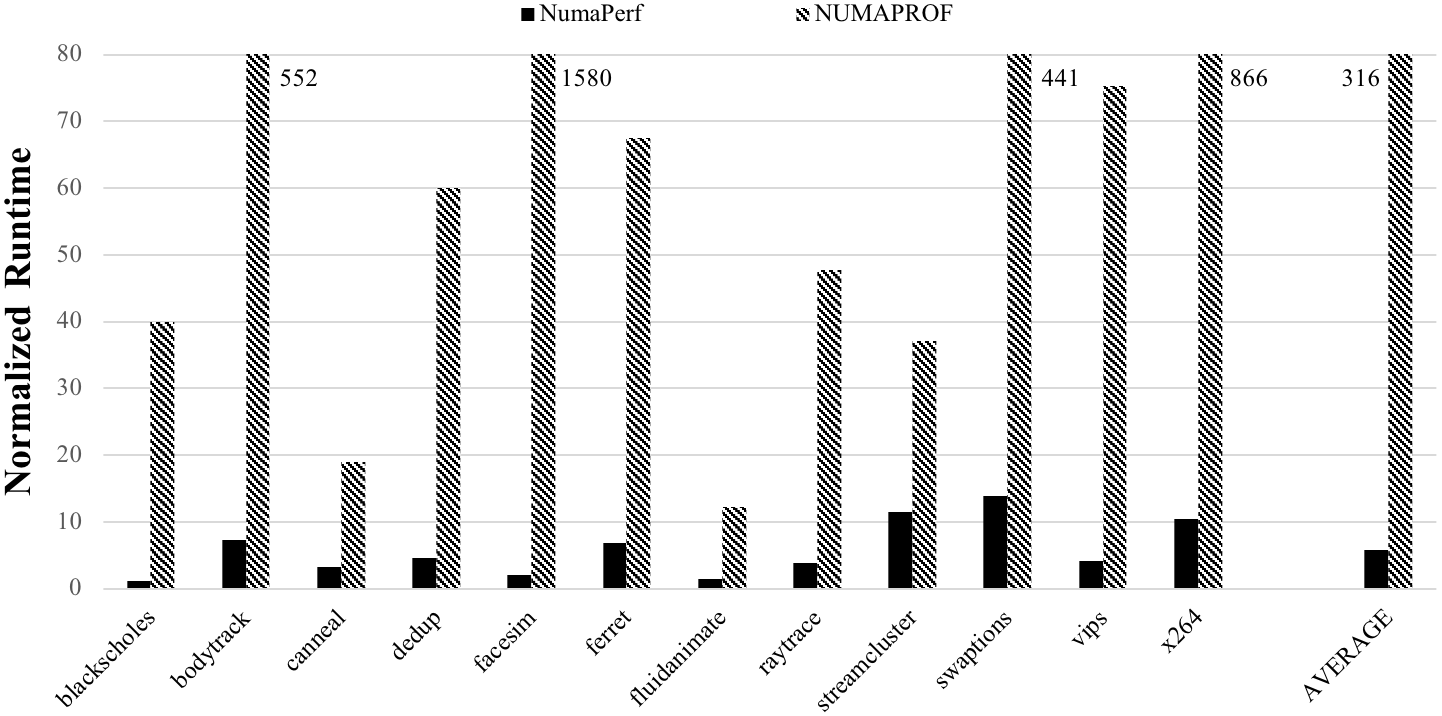
\includegraphics[width=3.2in]{paper/figures/performance.pdf}
    \caption{Performance overhead of \NP{} and others.\label{fig:performance}}  
\end{figure}
%\todo{xin new writing

We also evaluated the performance of \NP{} on PARSEC applications, and the performance results are shown in Figure~\ref{fig:performance}. On average, \NP{}'s overhead is around 585\%, which is orders-of-magnitude smaller than the state-of-the-art fine-grained profiler --- NUMAPROF~\cite{valat:2018:numaprof}. In contrast, NUMAPROF's overhead runs $316\times$ slower than the original one. \NP{} is designed carefully to avoid such high overhead, as discussed in Section~\ref{sec:implementation}. Also, \NP{}'s compiler-instrumentation also helps reduce some overhead by excluding memory accesses on stack variables. 

There are some exceptions. Two applications impose more than $10\times$ overhead, including Swaption and x264. Based on our investigation, the instrumentation with an empty function imposes more than $5\times$ overhead. The reason is that they have significantly more  memory accesses compared with other applications like blackscholes. Based on our investigation, swaption has more than $250\times$ memory accesses than  blackscholes in a time unit. Applications with low overhead can be caused by not instrumenting libraries, which is typically not the source of NUMA performance issues. 

%Besides, \NP{} has to do lots of computation inside the intercepting function which could make memory access go up to multiple times. And if a target application contains any NUMA issues, the issue also could arise in \NP{}. Based on this situation, we believe \NP{} did it very well to achieve a good performance. 

\subsection{Memory Overhead}
\label{sec:memory}
%\renewcommand{\arraystretch}{1.5}
\begin{table}[!htp]
% \footnotesize
% \setlength{\tabcolsep}{0.3em}
  \centering
    \begin{tabular}{|l|r|r|r|}
    \hline
    \multirow{2}{*}{Apps}&
    \multicolumn{3}{c|}{Memory Usage (MB)}\\
    \cline{2-4}
    &Glibc&\NP&NUMAPROF \\ \hline
    \hline
    blackscholes&617&689&685\\ \hline
    bodytrack&36&139&260\\ \hline
    canneal&887&1476&2383\\ \hline
    dedup&917&1806&2388\\ \hline
    facesim&2638&2826&3005\\ \hline
    ferret&160&301&445\\ \hline
    fluidanimate&470&667&753\\ \hline
    raytrace&1287&1610&2089\\ \hline
    streamcluster&112&216&928\\ \hline
    swaptions&28&67&255\\ \hline
    vips&226&283&463\\ \hline
    x264&2861&3039&3108\\ \hline \hline  
    Total&{\bf 10238}&{\bf 13120}&{\bf 16762}\cr\hline
    \end{tabular}
  \caption{Memory consumption of different profilers. \label{tab:memory_consumption}}
  \vspace{-0.2in}
\end{table}

We further evaluated \NP{}'s memory overhead with PARSEC applications. The results are shown in Table~\ref{tab:memory_consumption}. In total, \NP{}'s memory overhead is around 28\%, which is much smaller than the state-of-the-art fine-grained profiler --- NUMAPROF~\cite{valat:2018:numaprof}. \NP{}'s memory overhead is mainly coming from the following resources. First, \NP{} records the detailed information in page-level and cache-level, so that we could provide detailed information to assist bug fixes. Second, \NP{} also stores allocation callsites for every object in order to attribute performance issues back to the data. 

We  notice that some applications have a larger percentage of memory overhead, such as \texttt{streamcluster}. For it, a large object has very serious NUMA issues. Therefore, recording page and cache level detailed information contributes to the major memory overhead. However, overall, \NP{}'s memory overhead is totally acceptable, since it provides much more helpful information to assist bug fixes. 

%and thread based levels, especially \NP{} also provides lots of help information to help users fix the issues.
%Because \NP{} has to use lots of memory to record variety memory access patterns in all levels for potential issues. That is why some applications like bodytrack, dedup and streamcluster could get 2 times memory overheads.In these applications, they got some very huge objects with very serious NUMA issues ,like streamcluster contained an object that could occupy 100MB.To track the access pattern and provide detailed help information, doubled or more memory overheads are very reasonable.So to reduce memory overheads, \NP{} applied lots of mechanisms to avoid some objects if they look like not suspicious.That is why some applications like blackscholes, facesim and x264 bring very tiny memory overheads.Overall, \NP{} occupied less memory compared with NUMAPROF, but provided more information.

%\todo{Adding some explanation for memory utilization}. 

\subsection{Architecture Sensitiveness}
\label{sec:archindependent}

We further confirm whether \NP{} is able to detect similar performance issues when running on a non-NUMA or UMA machine. We further performed the experiments on a two-processor machine, where each processor is Intel(R) Xeon(R) Gold 6230 and each processor has 20 cores. We explicitly disabled all cores in node 1 but only utilizing 16 hardware cores in node 0. This machine has 256GB of main memory, 64KB L1 cache, and 1MB of L2 cache. The experimental results are further listed in Table~\ref{tab:independent}. For simplicity, we only listed the applications, the issue number, and serious scores in two different machines. 

Table~\ref{tab:independent} shows that most reported scores in two machines are very similar, although with small variance. The small variance could be caused by multiple factors, such as parallelization degree (concurrency). However, this table shows that all serious issues can be detected on both machines. This indicates that \NP{}  achieves its design goal, which could even detect NUMA issues without running on a NUMA machine. 

% \begin{table}[!htp]
% %\footnotesize
%  	\setlength{\tabcolsep}{0.3em}
% \centering
% \begin{tabular}{|c|l|l|r|r|}
%     \hline
%     \cline{1-5}
%     \multirow{2}{*}{Application}& \multicolumn{4}{c}{Specific Issues}\\
%     \cline{2-5}
%     & \# & Type & \multicolumn{1}{|c|}{\specialcell{Score\\(NUMA)}}  & \multicolumn{1}{|c|}{\specialcell{Score\\(UMA)}}\\ \hline

%     \multirow{2}{*}{AMG2006} & 1 & \PS & & \\
%     \cline{2-5}
    
%     &  2 &\TM&230 &\\ \hline

%     \multirow{7}{*}{lulesh}& 3 &\PS&1978&  \\
%     \cline{2-5}

%     &4&\PS&1611 &  \\
%     \cline{2-5}
    
%     &&5&\PS&1283&\multirow{2}{*}{lulesh.cc:2251-2264}&\BI&406\%&\multirow{2}{*}{418\%}& \\
%     \cline{3-5}\cline{7-8}\cline{10-10}
%     &&6&\FS&174&&\PAD &403\%&& \checkmark\\
%     \cline{3-10}
    
%     &&7&\PS&1316&\multirow{2}{*}{lulesh.cc:2089}&\BI&392\%&\multirow{2}{*}{407\%}& \\
%     \cline{3-5}\cline{7-8}\cline{10-10}
%     &&8&\FS&170&&\PAD &402\%&& \checkmark\\
%     \cline{3-10}
    
%     &&9&\TM&153&&\TB&\multicolumn{2}{|c|}{382\%}&\checkmark \\ \hline
    
%     UMT2013&131\%&10&\TM&253&&\TB&\multicolumn{2}{|c|}{131\%}&\checkmark \\
%     \hline 
%     \hline
    
%     \multirow{3}{*}{bodytrack}&\multirow{3}{*}{109\%}&11&\PS&10444&\multirow{2}{*}{FlexImageStore.h:146}&\PI&\multicolumn{2}{|c|}{\multirow{2}{*}{106\%}}& \\
%     \cline{3-5}\cline{7-7}\cline{10-10}
%     &&12&\FS&328&& &\multicolumn{2}{|c|}{}&\checkmark \\
%     \cline{3-10}
%     &&13&\TM&13646&&\TB&\multicolumn{2}{|c|}{105\%}&\checkmark \\ \hline
    
%     dedup&116\%&14&\TI&&& adjust threads  &\multicolumn{2}{|c|}{116\%}&\checkmark \\ \hline
    
%     facesim&105\%&15&\TM&399&&\TB&\multicolumn{2}{|c|}{105\%}&\checkmark \\ \hline
    
%     ferret&206\%&16&\TI&&& adjust threads  &\multicolumn{2}{|c|}{206\%}&\checkmark \\ \hline
 
%     \multirow{5}{*}{fluidanimate}&\multirow{5}{*}{429\%}&17&\PS&154&\multirow{2}{*}{pthreads.cpp:294}&\PI&112\%&\multirow{2}{*}{160\%}& \\
%     \cline{3-5}\cline{7-8}\cline{10-10}
%     &&18&\FS&223&&\PAD&158\%&&\checkmark \\
%     \cline{3-10}
    
%     &&19&\PS&45994&\multirow{2}{*}{pthreads.cpp:292}& \multirow{2}{*}{\PI} &\multicolumn{2}{|c|}{\multirow{2}{*}{340\%}}& \\
%     \cline{3-5} \cline{10-10}
%     &&20&\TS&19545&&&\multicolumn{2}{|c|}{}&\checkmark \\
%     \cline{3-10}
     
%     &&21&\TM&812&&\TB&\multicolumn{2}{|c|}{418\%}&\checkmark \\ \hline
    
%     \multirow{4}{*}{streamcluster}&\multirow{4}{*}{167\%}&22&\PS&405&\multirow{2}{*}{streamcluster.cpp:984}&\PI&100\%&\multirow{2}{*}{103\%}& \\
%     \cline{3-5}\cline{7-8}\cline{10-10}
%     &&23&\FS&368&&\PAD&102\%&& \checkmark\\
%     \cline{3-10}
     
%     &&24&\PS&6397&streamcluster.cpp:1845&\DUP&\multicolumn{2}{|c|}{158\%}& \\
%     \cline{3-10}
     
%     &&25&\TM&252&&\TB&\multicolumn{2}{|c|}{132\%}&\checkmark \\ \hline
%     \end{tabular}
%   \caption{Detected NUMA performance issues of \NP{}, where it detects 15 performance bugs that cannot be detected using existing NUMA profilers (with a check mark in the last column).}
%   \label{tab:independent}
% \end{table}

%\todo{Can not run UMT2013 successfully in UMA after a lot of efforts, need more time to fix}

\begin{table}[!htp]
%\footnotesize
 	\setlength{\tabcolsep}{0.45em}
\centering
\begin{tabular}{|c|l|l|l|l|}
\hline
\multirow{2}{*}{Application}  & \multicolumn{4}{c|}{Specific   Issues}                                                              \\ \cline{2-5} 
                              & \# & \multicolumn{1}{c|}{Type} & \multicolumn{1}{c|}{\specialcell{Score\\(NUMA)}} & \multicolumn{1}{c|}{\specialcell{Score\\(UMA)}} \\ \hline
\multirow{2}{*}{AMG2006}       & 1  & \PS     & 7390  & 5405  \\ \cline{2-5} 
                               & 2  & thread migration & 6     & 6      \\ \hline
\multirow{7}{*}{lulesh}        & 3  & \PS     & 1840  & 2443  \\ \cline{2-5} 
                               & 4  & \PS     & 1504  & 2353  \\ \cline{2-5} 
                               & 5  & \PS     & 4496  & 4326  \\ \cline{2-5} 
                               & 6  & false sharing    & 26    & 51   \\ \cline{2-5} 
                               & 7  & \PS     & 1229  & 2136  \\ \cline{2-5} 
                               & 8  & false sharing    & 12    & 27    \\ \cline{2-5} 
                               & 9  & thread migration & 3328  & 5213      \\ \hline
UMT2013                        & 10 & thread migration & 18    &      \\ \hline \hline
\multirow{3}{*}{bodytrack}     & 11 & \PS     & 10800 & 8203  \\ \cline{2-5} 
                               & 12 & false sharing    & 24    & 153   \\ \cline{2-5} 
                               & 13 & thread migration & 297   & 190   \\ \hline 
dedup                          & 14 & thread imbalance &   92:1:3    &  88:4:4     \\ \hline
facesim                        & 15 & thread migration & 607   & 274   \\ \hline
ferret*                          & 16 & thread imbalance &      &       \\ \hline
\multirow{5}{*}{fluidanimate} & 17 & \PS              & 90534                            & 15765 \\ \cline{2-5} 
                               & 18 & true sharing     & 2941  & 1753  \\ \cline{2-5} 
                               & 19 & \PS     & 180   & 95   \\ \cline{2-5} 
                               & 20 & false sharing    & 20    & 80    \\ \cline{2-5} 
                               & 21 & thread migration & 73    & 34    \\ \hline
\multirow{4}{*}{streamcluster} & 22 & \PS     & 427   & 270   \\ \cline{2-5} 
                               & 23 & false sharing    & 31    & 153   \\ \cline{2-5} 
                               & 24 & \PS     & 7169  & 10259 \\ \cline{2-5} 
                               & 25 & thread migration & 229   & 214   \\ \hline
\end{tabular}
  \caption{Evaluation on architecture Sensitiveness. We evaluated \NP{} on a non-NUMA (UMA) machine, which has very similar results as that on a NUMA machine. For \texttt{ferret}, \NP{} reports a proportion of  $3:2:48:75$ on the 8-node NUMA machine, and $5:4:50:77$ on the UMA machine. \label{tab:independent}}
  \vspace{-0.2in}
\end{table}





\section{Limitation}
\label{sec:discussion}
\NP{} bases on compiler-based instrumentation to capture memory accesses. Therefore, it shares the same shortcomings and strengths of all compiler-based instrumentation. On the one side, \NP{} can perform static analysis to reduce unnecessary memory accesses, such as accesses to stack variables. With static analysis, \NP{} typically achieves much better performance than binary-based instrumentation tools, such as NUMAPROF~\cite{valat:2018:numaprof}. On the other side, \NP{} requires the re-compilation (and the availability of the source code), and will miss memory accesses without the instrumentation. That is, it cannot detect NUMA issues caused by non-instrumented components (e.g., libraries), suffering from false negatives. 
In the future, we are planning to add binary-based instrumentation to \NP{} so that it could be utilized without the requirement of source code, and detect more potential issues caused by libraries (therefore reduce false negatives). 
%However, most issues should only occur in applications, but not libraries. 
%\todo{Mention that it is beneficial to combine two approaches together, which will be our future plan}. 

%\XZ{In our extensive evaluation, we did compiler-based instrumentation for most applications by only recompiling their source code without other dependent libraries. This could reduce lots of overheads caused by unnecessary instrumentation for memory accesses from third-party libraries. However as we can see from the evaluation section that it is effective to detect major issues and gets excellent improvements. But in few cases like dedup and UMT2013, this approach  could missed some useful information. One situation is that the compiler-based approach only supports some popular programming languages like C, C++ and etc, which depends on what compiler is used. So if certain languages used in the application that is not supported by the compiler, it could limit the use of this tool. For example, Fortran is used in the UMT2013 and LLVM does not support the transformation of Fortran codes, so that \NP{} can not do instrumentation of that part of code and no way to collect any useful information for that. And in some few cases, third-party libraries did lots of remote memory accesses, which will be ignored too. For instance in the dedup, it uses some local static libraries and there are lots of remote memory access happened inside that. If \NP{} did not compile the libraries, \NP{} can not report accurate information for its thread-imbalance issue.}
\section{Related Work}
\label{sec:related}

This section discusses NUMA-profiling tools at first, and then discusses other relevant tools and systems.
\subsection{NUMA Profiling Tools} 


%It only focuses on four memory-latency parameters: g, r, G and R, and focuses on the local/global/remote NUMA architecture, which is different from local/remote architecture of modern hardware. g is the latency of accessing a single word of  global memory. G is to move apage from global to a local memory or vice versa. \texttt{r} is to access a single word of remote memory, while  $R$ is go move a page from one local memory to another.the common is to utilize a record of the data references made by a parallel program to derive the cost analysis. We have different focuses with ~\cite{Bolosky:1991:NPR:106972.106994}, which is to model important aspect of real-world behavior, and then derive which NUMA placement policy can achieve better performance. Typically, this paper utilizes the offline analysis.  

\paragraph{Simulation-Based Approaches:}
 Bolosky et al. propose to model NUMA performance issues based on the collected trace, and then derive a better NUMA placement policy~\cite{Bolosky:1991:NPR:106972.106994}.
 NUMAgrind employs binary instrumentation to collect memory traces, and simulates cache activities and page affinity~\cite{NUMAGrind}. MACPO reduces the overhead of collecting memory traces and analysis by focusing on code segments that have known performance bottlenecks~\cite{MACPO}. That is, it typically requires programmer inputs to reduce its overhead.  Simulation-based approaches could be utilized for any architecture, which are very useful. However, they are typically extremely slow, with thousands of performance slowdown, which makes them un-affordable even for development phases. Further, they still require to evaluate the performance impact for a given architecture, which will significantly limit its usage. \NP{} utilizes a measurement based approach, which avoids significant performance overhead of simulation-based approaches. 

\paragraph{Fine-Grained Approaches:} 
TABARNAC focuses on the visualization of memory access behaviors of different data structures~\cite{TABARNAC}. It uses PIN to collect memory accesses of every thread on the page level, and then relates with data structure information together to visualize the usage of data structures. It introduces the runtime overhead between $10\times$ and $60\times$, in addition to its offline overhead. Diener et al. propose to instrument memory accesses with PIN dynamically, and then characterize distribution of accesses of different NUMA nodes~\cite{diener2015characterizing}. The paper does not present the detailed overhead. 
Numaprof also uses the binary instrumentation  (i.e., PIN) to collect and identify local and remote memory accesses~\cite{valat:2018:numaprof}. 
%\todo{Why NumaProf does not perform as good as \NP{}??? Are they helpful to identify the issues?} 
Numaprof relies on a specific thread binding to detect remote accesses, which shares the same shortcoming as other existing work~\cite{XuNuma, 7847070}. 
Numaprof also shares the same issues with other tools, which only focuses on remote accesses while omitting other issues such as cache coherence issues and imbalance issues. 
In addition, Numaprof is only a code-based profiler that could only report program statements with excessive remote memory access, which requires programmers to figure out the data (object) and a specific strategy. Due to this shortcoming, it makes the comparison with Numaprof extremely difficult and time-consuming. 
In contrast, although \NP{} also utilizes fine-grained measurement, it detects more issues that may cause performance issues in any NUMA architecture, and provides more useful information for bug fixes.    

%numap provides a cross-architecture APIs that enables to easily build profiling  tools~\cite{7818331}. 
% However, how they differentiate remote and local access is too week.They marked an access as remote access only if both threads and memories are explicitly binded by users and they happened to be pined to different nodes, unless they are counted as unpinned access.This mechanism is useless for the detection, since in most cases people do not do the binding explicitly by themselves.Further more, they only provide code centric metrics, which is helpless about where the memory is coming from and how to eliminate the detected issues.



\paragraph{Coarse-Grained Approaches:}
Many tools employ hardware Performance Monitoring Units (PMU) to identify NUMA-related performance issues, such as VTune~\cite{Intel:VTune}, Memphis~\cite{Memphis}, MemProf~\cite{Lachaize:2012:MMP:2342821.2342826}, Xu et al.~\cite{XuNuma}, NumaMMA~\cite{NumaMMA}, and LaProf~\cite{7847070}, where their difference are further described in the following. 
Both VTune~\cite{Intel:VTune} and Memphis~\cite{Memphis} only detects NUMA-performance issues on statically-linked variables.  
MemProf proposes the employment of hardware Performance Monitoring Units (PMU) to identify NUMA-related performance issues~\cite{Lachaize:2012:MMP:2342821.2342826}, with the focus on remote accesses. It constructs data flow between threads and objects to help understand NUMA performance issues. One drawback of MemProf is that it requires an additional kernel module that may prevent people of using it. Similarly, Xu et al. also employ PMU to detect NUMA performance issues~\cite{XuNuma}, but without the change of the kernel. It further proposes a new metric-- the NUMA latency per instruction--to evaluate the seriousness of NUMA issues, which helps to filter out non-serious NUMA issues. However, this tool has a drawback that it statically binds every thread to each node, which may miss some NUMA issues due to its static binding. 
NumaMMA also collects traces with PMU hardware, but focuses on the visualization of memory accesses ~\cite{NumaMMA}. LaProf focuses on multiple issues that may cause performances issues in NUMA architecture~\cite{7847070}, including data sharing, shared resource contention, and remote imbalance. LaProf has the same shortcoming by binding every thread statically.  Overall, these sampling-based approaches although imposes much lower overhead, making them applicable even for the production environment, they cannot detect all NUMA performance issues especially when most of them only focus on remote accesses. In contrast, \NP{} aims to detect performance issues inside  development phases, avoiding any additional runtime overhead. Also, \NP{} focuses more aspects with a predictive approach, not just limited to remote accesses in the current hardware. Our evaluation results confirm \NP{}'s comprehensiveness and effectiveness. 

%Xu's work is sampling based,and for each memory access sampling event,it identifies whether it is a remote memory access or not according to the NUMA node id and the location of the target memory. For remote access, they will further get the memory access latency which is supported by hardware sampling like IBS and PEBS-LL.Overall, they can identify NUMA issues if the average NUMA remote memory access latency per instruction is exceeding a threshold. Besides, they also provide memory access pattern across threads, which could be used to guide how to distribute memory to eliminate remote latency for users. However, the sampling method missed lots of information and potential NUMA issues which can be demonstrated based on our experiments. Further more, it does not support cache level contention problems and also thread based problems, so that users can get limited help information about the reasons of the detected issues and how to fix them. 
%Some of this fact are caused by their implementation. For instance, in order to reduce the overhead of identifying the thread location, some tools bind every thread to a specific node that allows to infer the thread node using a thread-private variables~\cite{XuNuma}, instead of employing a system call.  However, they may miss some issues due to their binding. 




\subsection{Other Related Tools}
RTHMS also employs PIN to collect memory traces, and then assigns a score to each object-to-memory based on its algorithms~\cite{RTHMS}. It aims for identifying the peformance issues for the hybrid DRAM-HBM architecture, but not the NUMA architecture, and has a higher overhead than \NP{}. Some tools focus on the detection of false/true sharing issues~\cite{Sheriff, Predator, Cheetah, DBLP:conf/ppopp/ChabbiWL18, helm2019perfmemplus}, but skipping other NUMA issues. 

SyncPerf also detects load imablance and predicts the optimal thread assignment~\cite{SyncPerf}. SyncPerf aims to achieve the optimal thread assignment by balancing the waiting time of each types of threads. In contrast, \NP{} suggests the optimal thread assignment based  the number of accesses of each thread, which indicates the actual workload. 

%Predator\cite{Predator} also used emulation based approach to detect false problems, which is very similar with NumaPerf. By emulate cache line, they could collection some information like when did a cache invalidation happened, how the cache line is shared between threads:true sharing or false sharing, and also how serious the sharing is. But this work is mainly focus on false sharing issues detection, which did not take NUMA perspectives into consider.


%\paragraph{Compiler-assisted Instrumentation}



\section{Conclusion}
\label{sec:conclusion}

Parallel applications running on NUMA machines are prone to different types of performance issues. Existing NUMA profilers may miss significant portion of optimization opportunities. Further, they are bound to a specific NUMA topology. Different from them, \NP{} proposes an architecture-independent  and scheduling-independent method that could detect NUMA issues even without running on a NUMA machine. Comparing to existing NUMA profilers, \NP{} detects more performance issues without false alarms, and also provides more helpful information to assist bug fixes. In summary, \NP{} will be an indispensable tool that could identify NUMA issues in development phases. 


%-------------------------------------------------------------------------------
\bibliographystyle{plain}
\bibliography{refs,tongping}

%%%%%%%%%%%%%%%%%%%%%%%%%%%%%%%%%%%%%%%%%%%%%%%%%%%%%%%%%%%%%%%%%%%%%%%%%%%%%%%%
\end{document}
%%%%%%%%%%%%%%%%%%%%%%%%%%%%%%%%%%%%%%%%%%%%%%%%%%%%%%%%%%%%%%%%%%%%%%%%%%%%%%%%

%%  LocalWords:  endnotes includegraphics fread ptr nobj noindent
%%  LocalWords:  pdflatex acks